\chapter{Eventos,cultura e lazer}
\DoPToC
\section{Apresentação}

E aí calouros, beleza? Então, você que começou agora e tá achando que faculdade é puro estudo, que você vai ter que deixar de aproveitar seu tempo livre pra ficar estudando feito um maluco, fazendo de tudo para conseguir um rendimento bom, mas não é bem assim que funciona. Claro, estudar e conseguir notas boas é importante, mas a vida também tem de ser aproveitada, não é mesmo? Você vai descobrir que na faculdade existem várias formas de lazer para você relaxar de todo o estresse, eventos relacionados a cultura para que você amplie seus conhecimentos sobre as mais variadas coisas e eventos para você competir e se divertir!     

\subsection{Eventos} 

A Enecomp (Encontro Nacional dos Estudantes de computação) é um evento organizado pelo Enec que conta com a participação de professores e pessoas que trabalham na área de computação tratando de diversos assuntos do interesse de nós alunos! Bem legal hein?

Para participar o aluno precisa entrar no site e preencher a ficha e efetuar o pagamento do ingresso. Infelizmente ainda não foram divulgadas mais informações a respeito de local e data sobre o evento deste ano. Para mais informações acesse o site: http://www.enec.org.br/EneComp

\subsection {SEMCOMP}
A Semcomp, como seu próprio nome diz, nada mais é que a semana da computação. Ela é realizada uma vez por ano e tem como objetivo fomentar o empreendedorismo tecnológico regional. Também conta com a participação de vários palestrantes para informar melhor sobre a área de computação. 

\subsection {Maratona de Progamação}
                \begin{wrapfigure}{R}{0.4\textwidth}
	                    \centering
                        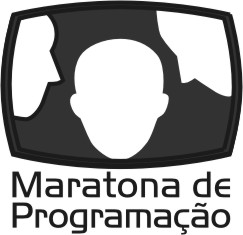
\includegraphics[width=0.39\textwidth]{MaratonadeProgramacao}
                     \end{wrapfigure}  

A Maratona de Programação é um evento bem divertido de se participar, pois é uma competição entre grupos de alunos para resolverem problemas através da programação. Seu objetivo é reunir equipes de 2 ou 3 alunos para participarem do campeonato mundial, o ICPC (International Collegiate Programming Contest). A competição é feita em duas etapas: A primeira é uma etapa regional visando selecionar os melhores grupos de cada região do Brasil. Ela acontecerá no dia 10 de setembro. Após realizada a primeira etapa, temos a etapa nacional, para selecionar os melhores grupos do Brasil inteiro. Essa segunda etapa acontecerá nos dias 11 e 12 de Novembro, em Belo Horizonte.

	Para participar o grupo de alunos deve passar pelo processo de seleção aqui mesmo na faculdade ou então o grupo poderá pagar uma taxa de inscrição (Passar na seleção sai mais barato hein!). Vocês não vão querer perder essa oportunidade única! Para mais informações acessem o site: http://maratona.ime.usp.br
    
\subsection {Olimpíada de computação} 
                 \begin{wrapfigure}{R}{0.3\textwidth}
	                    \centering
                        
\includegraphics[width=0.29\textwidth]{obi}
                     \end{wrapfigure}  

Aproveita sua chance que só alunos cursando o primeiro e segundo semestres pela primeira vez podem participar desse! A OBC conta com provas de níveis que vão desde o fácil, para aqueles que tem baixo conhecimento na área de computação até níveis difíceis, para aqueles com conhecimentos mais avançados de estrutura de dados.

	            A do ano de 2016 já passou e a data e o local de 2017 ainda não foram divulgados e nem como participar do evento. Para quem quiser saber mais e ficar atento ao site para quando as inscrições 
	            estiverem abertas acessem: http://olimpiada.ic.unicamp.br/info/geral.

\subsection {IEEEXTREME} 

O IEEEXTREME é um evento anual de competição de programação. O evento consiste em grupos de alunos resolvendo problemas relacionados a programação 24 horas em um dia.

\section{Cultura e lazer}
	            \subsection{Apresentação}
	                Já deu pra ter uma boa ideia da quantidade de coisa que se pode fazer na faculdade para ampliar seus conhecimentos e ao mesmo tempo se divertir na faculdade não é mesmo? Mas que tal relaxar e aprender sobre novas culturas? Vou listar para vocês algumas coisas que acontecem por aqui:

\subsection {Prática do Corpo}

Consiste na prática de dança radial e acroyoga.  Tudo que o aluno precisa fazer é se inscrever. Acontece no patio da Escola de Dança UFBA na sala 04, segundas e quartas das 14h às 16h. Para saber mais, vá até o PAF IV.

\subsection {Curso de Dança Contemporâneo}

O lema do curso é: "Um jeito de ser e de se mover brasileiro".Como o próprio lema diz se trata da musicalidade afro-brasileira e seus ritmos. Para participar o aluno precisa pagar uma taxa de 50 reais por mês. O curso é realizado no portão principal da UFBA, em frente a entrada para o jardim zoológico. Para mais informações, vá até o PAF IV.

\subsection {Escola de Teatro}

\begin{wrapfigure}{R}{0.4\textwidth}
	\centering	\includegraphics[width=0.39\textwidth]{teatro}
\end{wrapfigure}

A escola de Teatro da UFBA tem o objetivo de divulgar a dramaturgia contemporânea com a implantação de um instituto-modelo onde se formam atores, diretores e professores com os mais modernos métodos e técnicas. 

Além de promover a integração efetiva da produção universitária com a vida cultural da comunidade. Bem legal não é mesmo?

A escola se encontra na Av. Araújo Pinho, 292, Canela, Salvador – BA. Para mais informações ligue (71) 3283-7044.

\subsection {Museu de Arqueologia e Etnologia}
\begin{wrapfigure}{R}{0.5\textwidth}
	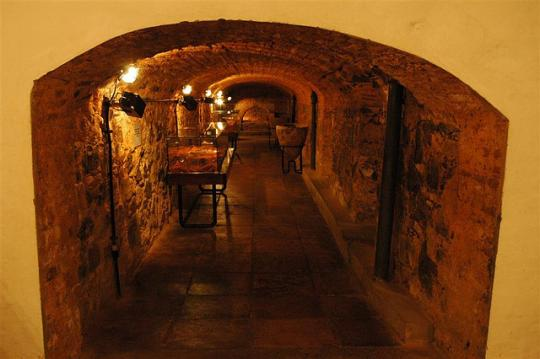
\includegraphics[width=0.49\textwidth]{museuarq}
\end{wrapfigure}  

O Museu de Arqueologia e Etnologia ou MAE representa os mais completos vestígios arquitetônicos do Colégio dos Jesuítas. Busca preservar e reconstituir a memória e identidade do povo brasileiro através de suas exposições de acervos arqueológicos e etnográficos. Ele se encontra no Largo Terreiro de Jesus, S/N, Pelourinho, Salvador - BA. O ingresso custa 6 reais a inteira e é gratuito para crianças até 5 anos, estudantes e professores da Rede Pública e Comunidade UFBA. Para mais informações: (71) 3283-5540.
                    
\subsection {Museu Afro Brasileiro}  

O museu Afro Brasileiro trata exclusivamente das culturas africanas e sua presença na formação da cultura brasileira. O museu se encontra no Largo Terreiro de Jesus, S/N, Pelourinho, Salvador - BA. O ingresso custa 6 reais a inteira e é gratuito para crianças até 5 anos, estudantes e professores da Rede Pública e Comunidade UFBA. Para mais informações: (71) 3283-5540.
                    
\subsection {Museu de Geologia} 
                    
Uma visita ao Museu Geológico da Bahia é um convite a conhecer o solo e as rochas onde pisamos, as riquezas do subsolo, bem como os fósseis dos seres que habitaram a nossa Terra. Possui um dos maiores acervos de rochas, de minerais, de pedras preciosas e de fósseis da Bahia, com mais de 20 mil peças, proporcionando aos seus visitantes uma viagem no tempo geológico através das suas exposições temáticas. Massa né não?
                	A entrada para o museu é gratuita e seus horários de visitação são:
	                De segunda a sexta, das 13h às 18h.
	                Aos sábados e domingos, das 13h às 17h.
	                O museu fica na Avenida Sete de Setembro, 2195, Corredor da Vitória.
                    Para mais informações acesse o site do museu: http://www.mgb.ba.gov.br/
	                \newpage
	            \section{Pontos turísticos de Salvador}
	                
	                 Além das opções proporcionadas diretamente pela UFBA, há varios lugares de salvador que valem a pena visitar. Entre eles temos:
	                 
\subsection {Praia Farol da Barra} 
\begin{wrapfigure}{R}{0.34\textwidth}
\centering                        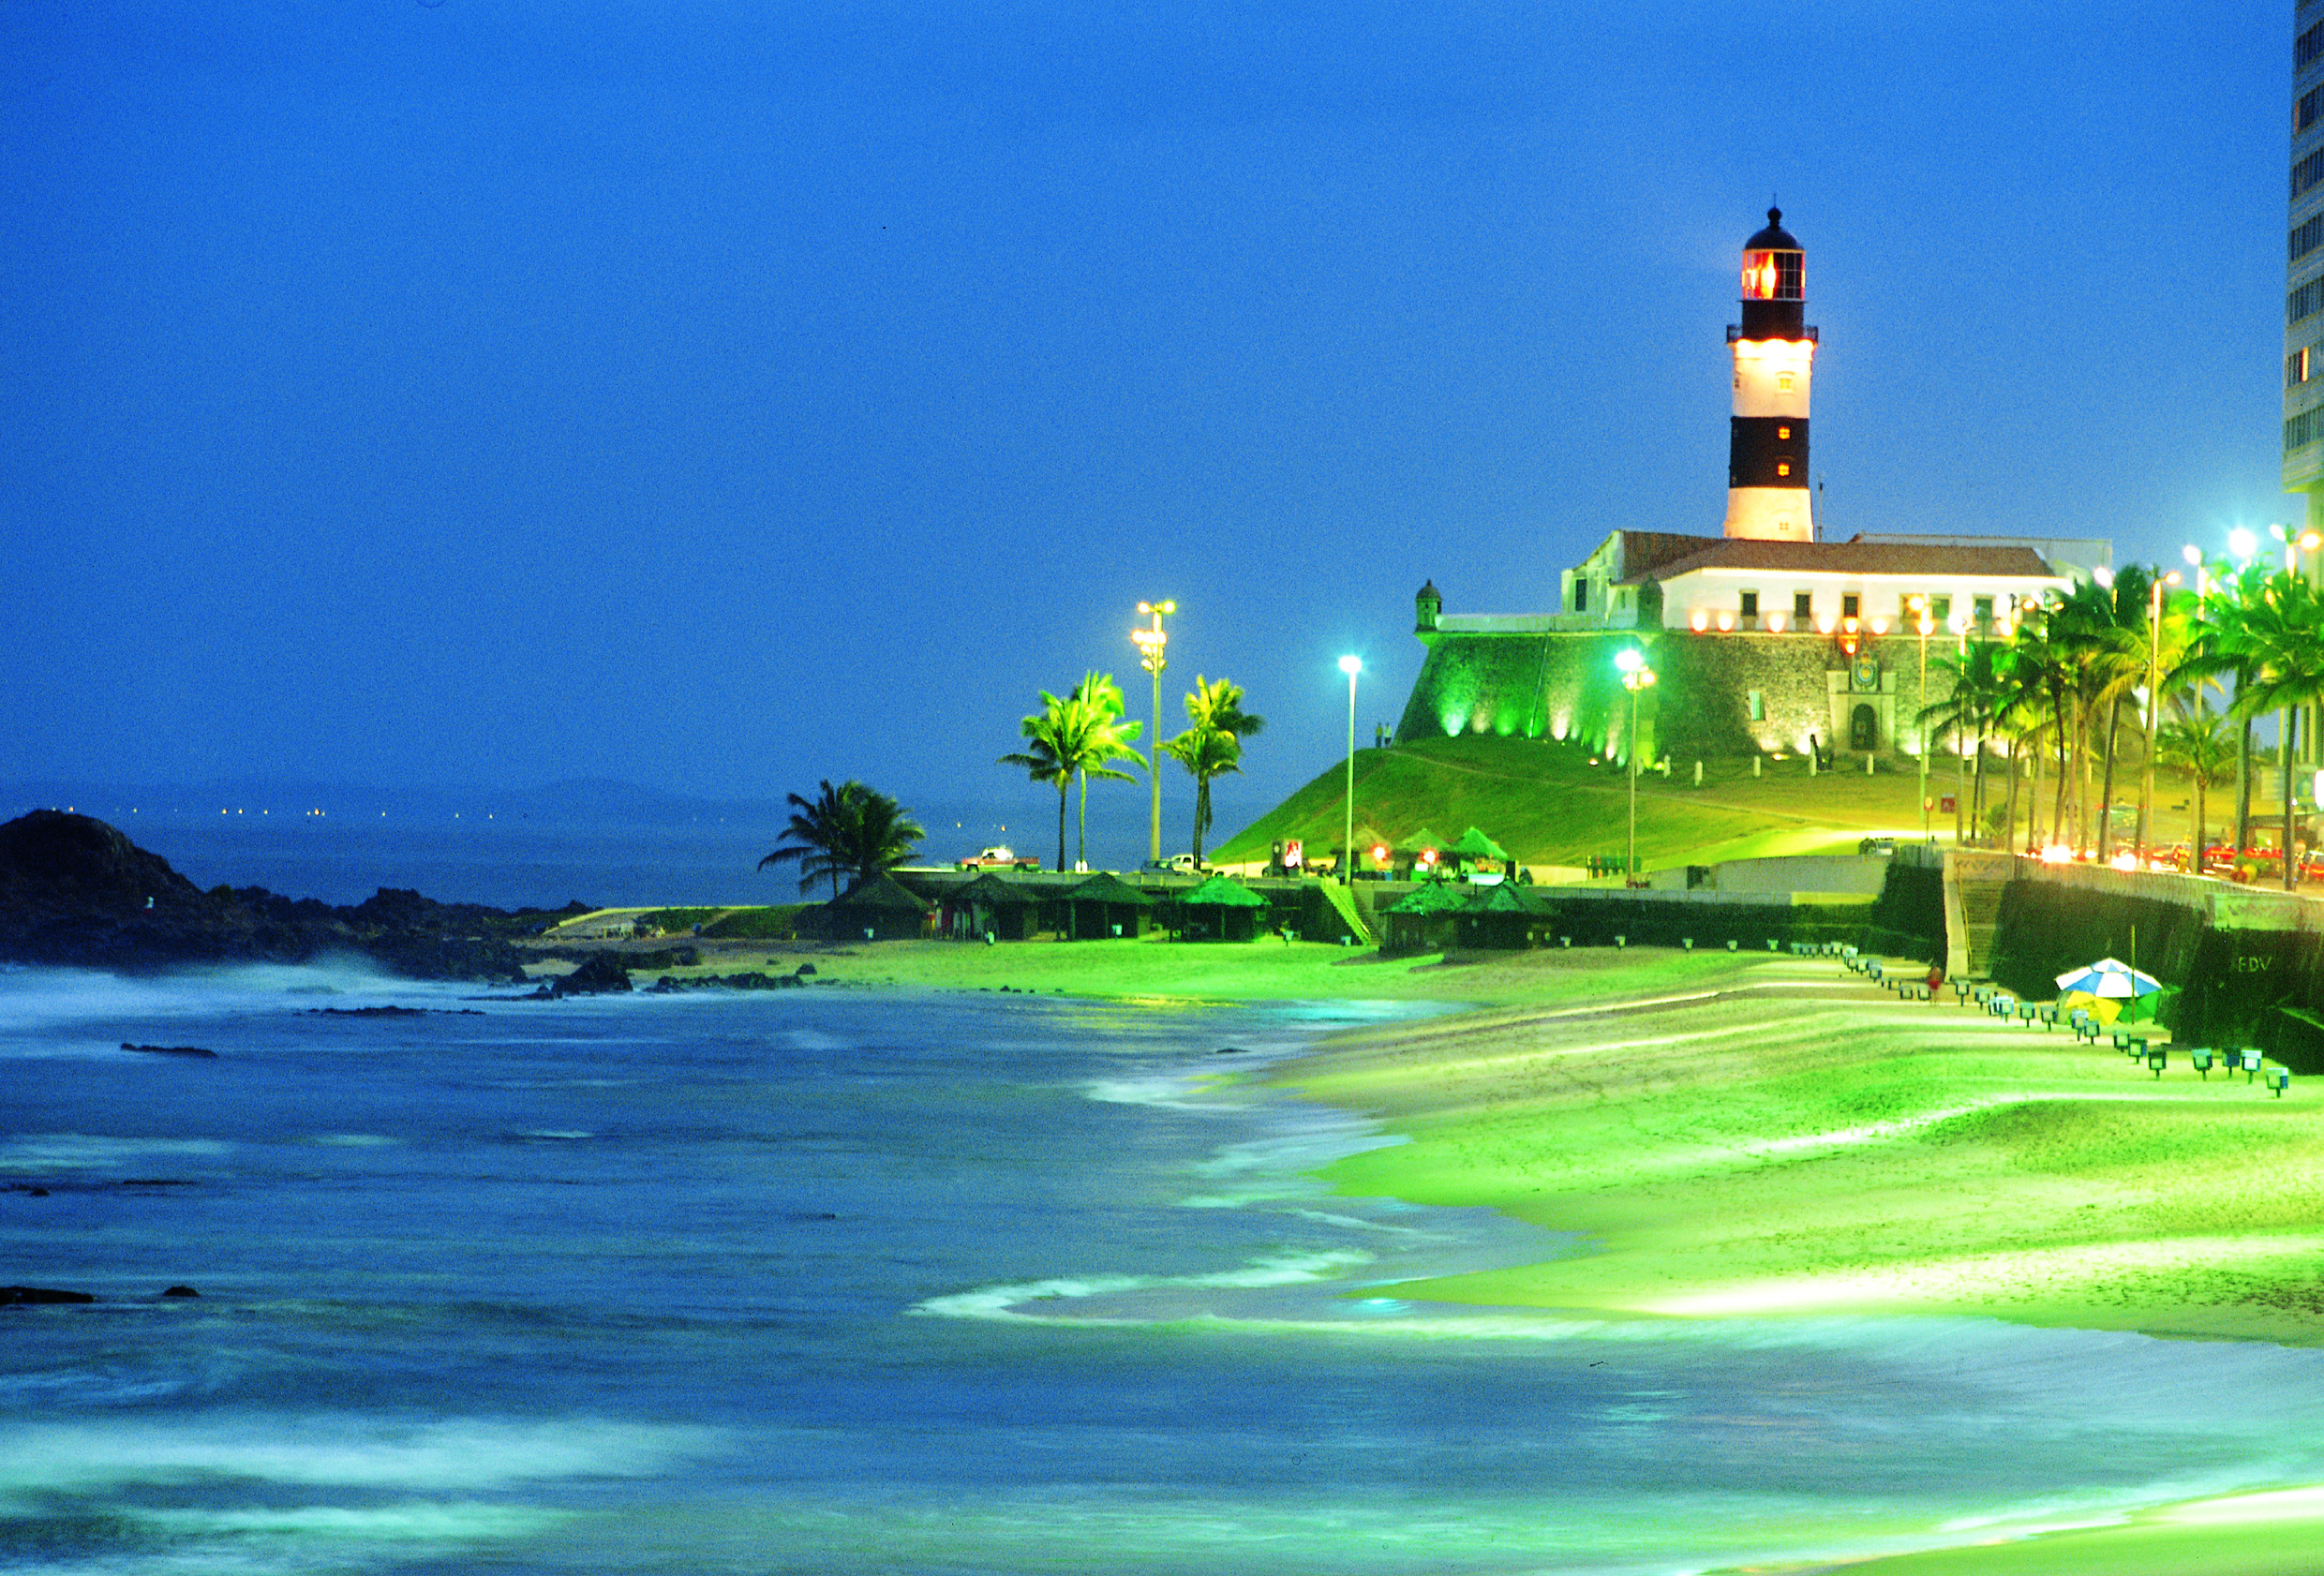
\includegraphics[width=0.33\textwidth]{faroldabarra}                        \end{wrapfigure}

Praia de águas tranquilas, de fácil acesso. Um dos melhores lugares para se observar o por do sol. 

A vista é magnífica e com conteúdo histórico. No farol existe o Museu Náutico da Bahia, reunindo um valioso acervo arqueológico submarino, uma coleção de instrumentos de navegação, entre outras coisas. 

A praia se encontra na Barra, inicia junto ao Farol da Barra, se estendendo até o morro do Cristo.
                          
\subsection {Igreja de Nosso Senhor do Bonfim}

Interessante templo católico, construido em estilo neoclássico com fachada e rococó. A igreja é conhecida pelas famosas fitinhas do Bonfim, e pela Lavagem do Bonfim, festa realizada uma vez por ano no local. Fica localizada na Sagrada Colina, na península de Itagipe.

\subsection {Teatro Castro Alves}       \begin{wrapfigure}{L}{0.34\textwidth}
\centering     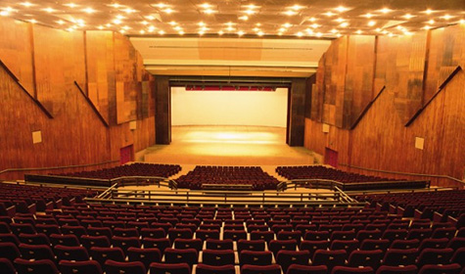
\includegraphics[width=0.33\textwidth]{img-18-big}
\end{wrapfigure}   
                     Maior e mais importante centro artístico da cidade. Nele são realizados diversas apresentações teatrais com frequência e até mesmo shows de música. 
                     
Artistas como Raul Seixas, Gilberto Gil, Chico Buarque, entre outros se destacam entre os que já se apresentaram no TCA(Teatro Castro Alves). 

O teatro é localizado no bairro do Campo Grande, na praça Dr. Mario Macedo Costa.

\subsection {Pelourinho}
                      \begin{wrapfigure}{R}{0.4\textwidth}
	                    \centering
                        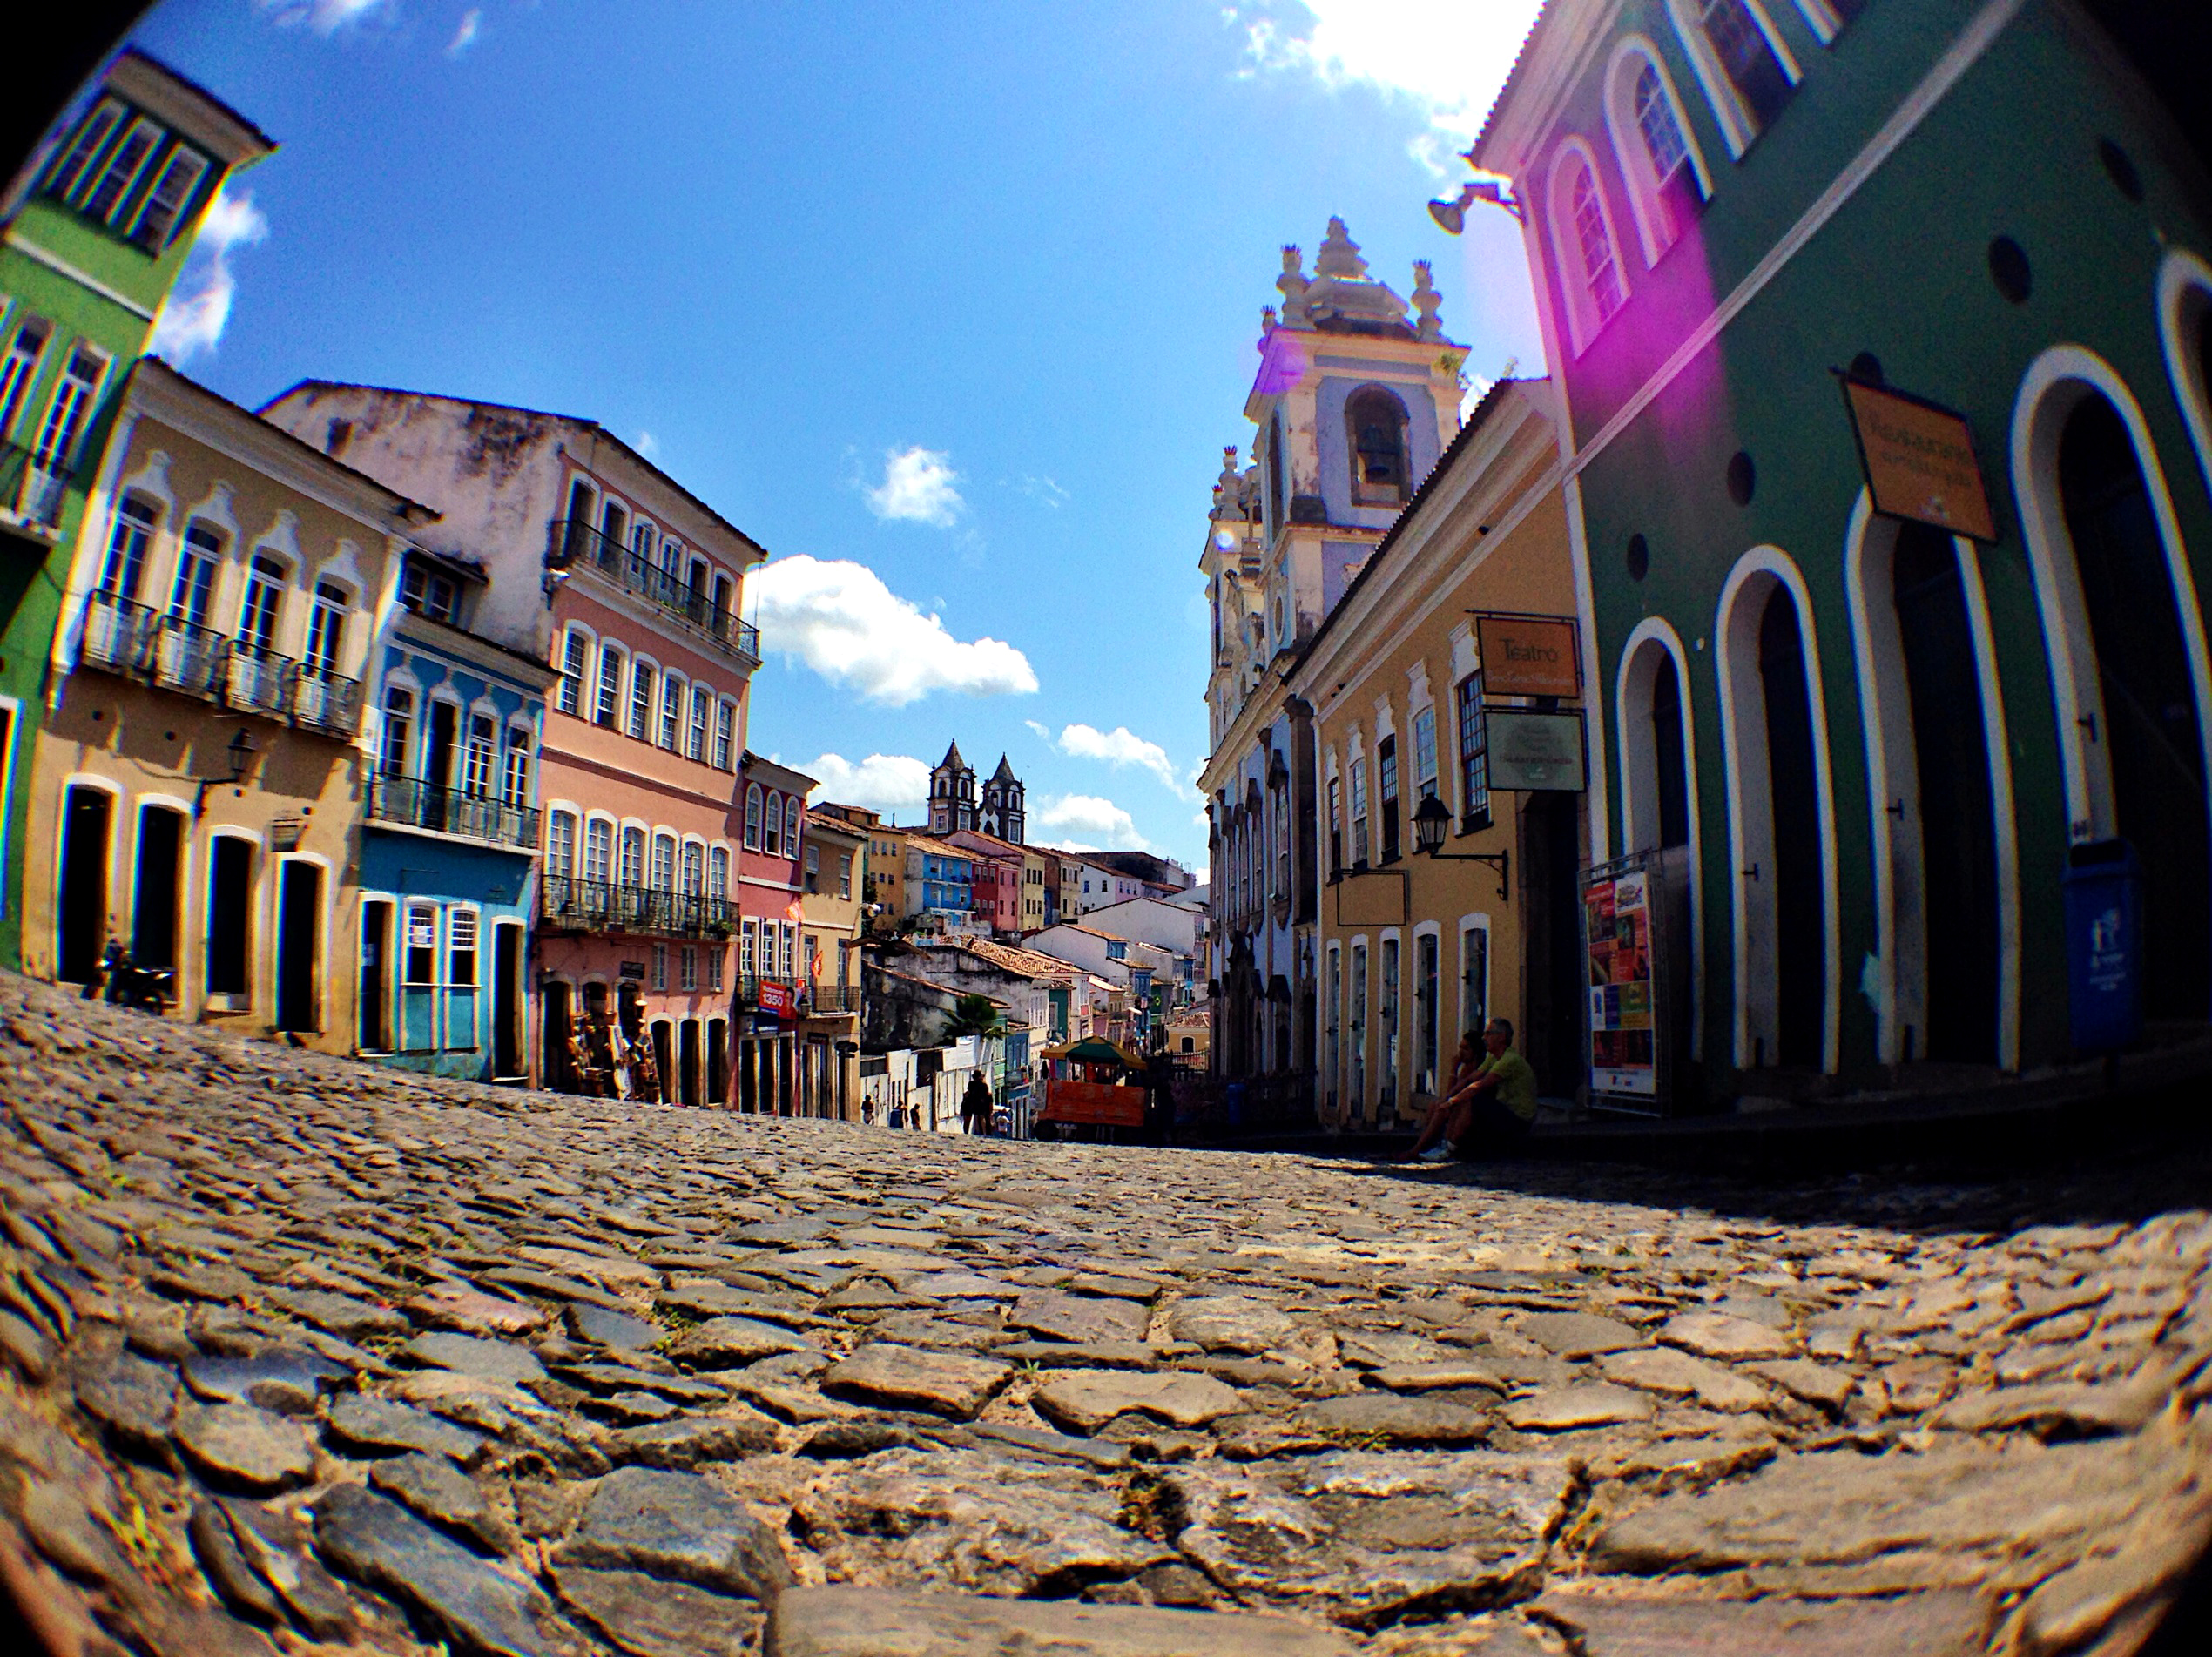
\includegraphics[width=0.39\textwidth]{Largo_do_Pelourinho_-_Salvador}
                     \end{wrapfigure} 
                     
Considerado como o “coração da cidade” e conhecido como o centro da cultura africana do Brasil, o pelourinho conta com casarões coloridos, igrejas, lojas e restaurantes. Carros não entram nessa parte da cidade e só é possível se locomover a pé. Dentro do pelourinho fica localizado alguns dos museus citados anteriormente. Além do Convento de São Francisco, o qual tem o interior todo em ouro. 
                    
                     
               
 





     
     
     
     
     
     
     
     
     
     
     
     
     
     
     
     
     
     
     
     
     
     
     
     
     
     
     
     
     








